%%%%%%%%%%%%%%%%%%%%%%%%%%%%%%%%%%%%%
%                                   %
% Compile with XeLaTeX and biber    %
%                                   %
% Questions or comments:            %
%                                   %
% joshua dot mcneill at uga dot edu %
%                                   %
%%%%%%%%%%%%%%%%%%%%%%%%%%%%%%%%%%%%%

\documentclass{beamer}
  % Read in standard preamble (cosmetic stuff)
  %%%%%%%%%%%%%%%%%%%%%%%%%%%%%%%%%%%%%%%%%%%%%%%%%%%%%%%%%%%%%%%%
% This is a standard preamble used in for all slide documents. %
% It basically contains cosmetic settings.                     %
%                                                              %
% Joshua McNeill                                               %
% joshua dot mcneill at uga dot edu                            %
%%%%%%%%%%%%%%%%%%%%%%%%%%%%%%%%%%%%%%%%%%%%%%%%%%%%%%%%%%%%%%%%

% Beamer settings
% \usetheme{Berkeley}
\usetheme{CambridgeUS}
% \usecolortheme{dove}
% \usecolortheme{rose}
\usecolortheme{seagull}
\usefonttheme{professionalfonts}
\usefonttheme{serif}
\setbeamertemplate{bibliography item}{}

% Packages and settings
\usepackage{fontspec}
  \setmainfont{Charis SIL}
\usepackage{hyperref}
  \hypersetup{colorlinks=true,
              allcolors=blue}
\usepackage{graphicx}
  \graphicspath{{../../figures/}}
\usepackage[normalem]{ulem}
\usepackage{enumerate}

% Document information
\author{M. McNeill}
\title[FREN2001]{Français 2001}
\institute{\url{joshua.mcneill@uga.edu}}
\date{}

%% Custom commands
% Lexical items
\newcommand{\lexi}[1]{\textit{#1}}
% Gloss
\newcommand{\gloss}[1]{`#1'}
\newcommand{\tinygloss}[1]{{\tiny`#1'}}
% Orthographic representations
\newcommand{\orth}[1]{$\langle$#1$\rangle$}
% Utterances (pragmatics)
\newcommand{\uttr}[1]{`#1'}
% Sentences (pragmatics)
\newcommand{\sent}[1]{\textit{#1}}
% Base dir for definitions
\newcommand{\defs}{../definitions}


  % Packages and settings

  % Document information
  \subtitle[Femmes et questions]{Les femmes et les questions}

\begin{document}
  % Read in the standard intro slides (title page and table of contents)
  \begin{frame}
    \titlepage
    \tiny{Office: % Basically a variable for office hours location
Gilbert 121\\
          Office hours: % Basically a variable for office hours
 lundi, mercredi, vendredi 10:10--11:10
}
  \end{frame}

  \begin{frame}{Annonces}
    \begin{itemize}
      \item Le devoir 2 à rendre le 23 septembre.
      \item[] \tinygloss{Homework 2 to be turned in September 23rd.}
    \end{itemize}
  \end{frame}

  \begin{frame}{Un adjectif masculin ou féminin?}
    \begin{center}
      Camille est \underline{\uncover<2->{amusan\sout{t}}} \\
      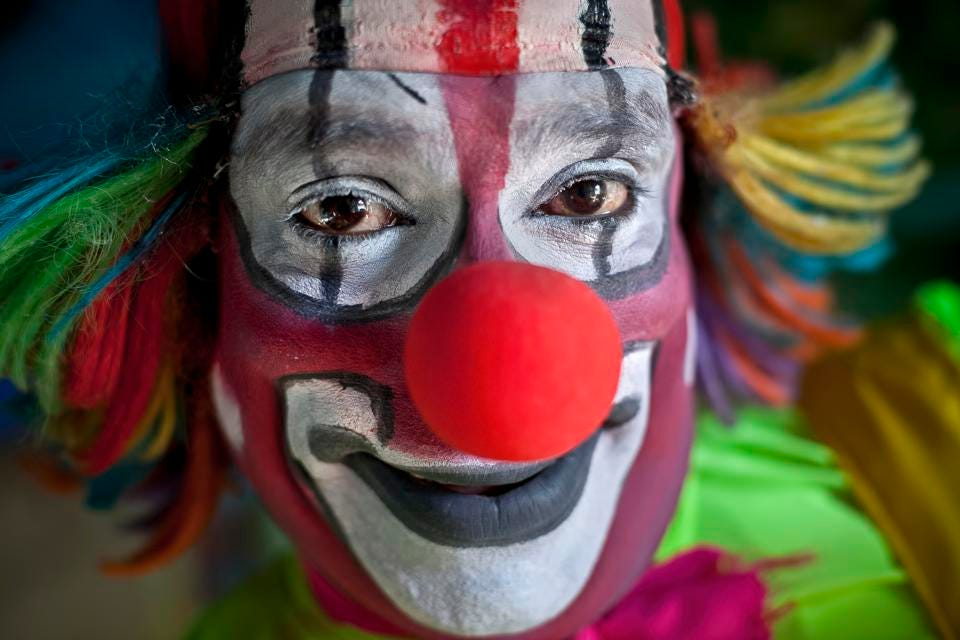
\includegraphics[scale=0.25]{clown.jpg}
    \end{center}
  \end{frame}

  \begin{frame}{Un adjectif masculin ou féminin?}
    \begin{center}
      Sacha est \underline{\uncover<2->{gro\sout{s}}} \\
      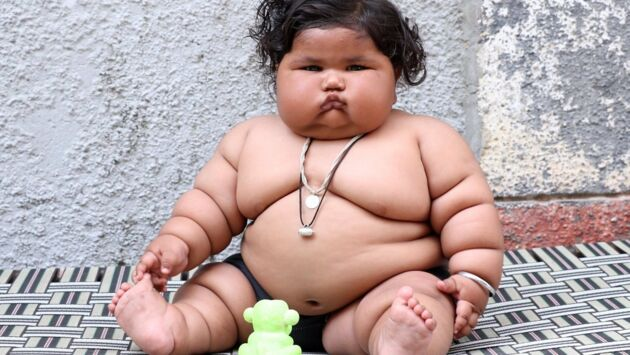
\includegraphics[scale=0.45]{gros.jpg}
    \end{center}
  \end{frame}

  \begin{frame}{Un adjectif masculin ou féminin?}
    \begin{center}
      Éloi est \underline{\uncover<2->{intelligen\alert{te}}} \\
      
\includegraphics[scale=0.5]{intelligente.jpg}
    \end{center}
  \end{frame}

  \begin{frame}{Un adjectif masculin ou féminin?}
    \begin{center}
      Laurence est \underline{\uncover<2->{ambitieu\alert{se}}} \\
      
\includegraphics[scale=0.4]{ambitieuse.jpg}
    \end{center}
  \end{frame}

  \begin{frame}{Un adjectif masculin ou féminin?}
    \begin{center}
      Patrice est \underline{\uncover<2->{blon\sout{d}}} \\
      
\includegraphics[scale=0.75]{blond.jpg}
    \end{center}
  \end{frame}

  \begin{frame}{Un adjectif masculin ou féminin?}
    \begin{center}
      Ange est \underline{\uncover<2->{bru\alert{ne}}} \\
      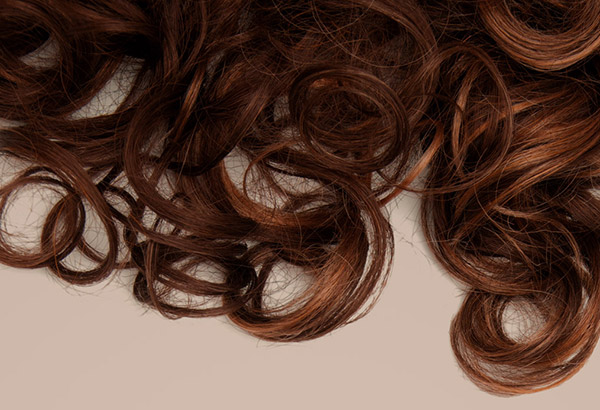
\includegraphics[scale=0.4]{brune.jpg}
    \end{center}
  \end{frame}

  \begin{frame}{}
    \begin{center}
      \Large Quiz
    \end{center}
  \end{frame}

  \begin{frame}{Entrevue}
    Trouvez un(e) camarade de classe avec qui vous n'avez pas encore parlé. Avec ce partenaire, faites des entrevues en posant des questions aux sujets suivants. \\
    \tinygloss{Find a classmate with whom you have not yet spoken. With this partner, interview each other by asking questions about the following subjects.}
    \begin{columns}
      \column{0.5\textwidth}
        \begin{enumerate}
          \item les amis
          \item la musique
          \item le sport
          \item les animaux
        \end{enumerate}
      \column{0.5\textwidth}
        Des mots interrogatifs:
        \begin{itemize}
          \item \lexi{est-ce que} (for yes/no questions)
          \item \lexi{qu'est-ce que} \gloss{what}
          \item \lexi{qui, qui est-ce que} \gloss{who}
          \item \lexi{comment} \gloss{how}
          \item \lexi{où} \gloss{where}
          \item \lexi{pourquoi} \gloss{why}
          \item \lexi{combien de} \gloss{how many}
        \end{itemize}
    \end{columns}
  \end{frame}

  \begin{frame}{Des traits opposés}
    Tes amis sont...
    \begin{enumerate}
      \item méchants $\to$ \underline{\uncover<2->{gentils}}
      \item égoïstes $\to$ \underline{\uncover<3->{généreux}}
      \item bêtes $\to$ \underline{\uncover<4->{intelligents}}
      \item sédentaires $\to$ \underline{\uncover<5->{énergiques}}
      \item paresseux $\to$ \underline{\uncover<6->{ambitieux}}
      \item sérieux $\to$ \underline{\uncover<7->{drôle}}
      \item mal habillés $\to$ \underline{\uncover<8->{élégants}}
      \item laids $\to$ \underline{\uncover<9->{beaux}}
    \end{enumerate}
  \end{frame}

  \begin{frame}{}
    \begin{center}
      \Large Questions?
    \end{center}
  \end{frame}
\end{document}
